\section{Experiments}
\label{sec:experiments}

% Declare experiment figures before the prose so two-column floats enter the
% placement queue early.
\begin{figure*}[!t]
\centering
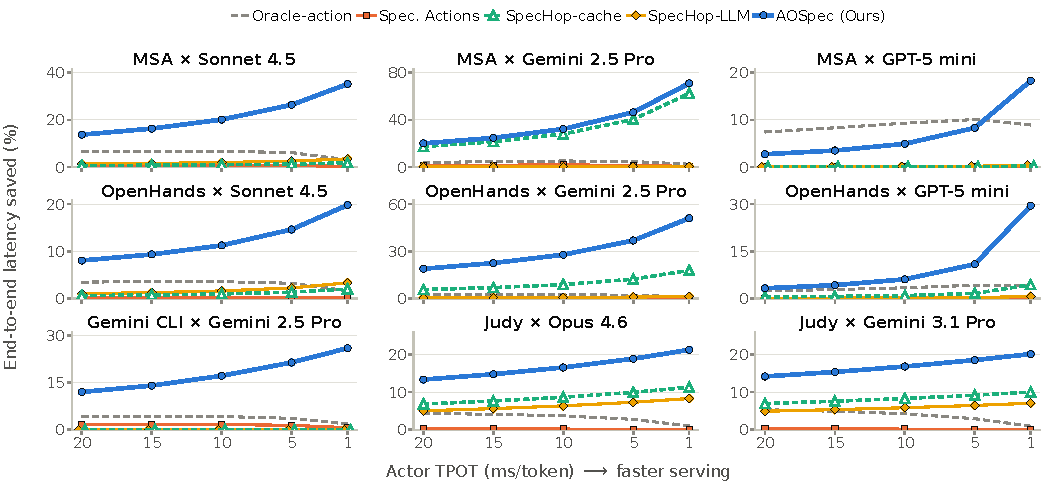
\includegraphics[width=\textwidth]{figs/grid_tpot_lines}
\caption{End-to-end latency savings across nine Terminal-Bench harness and actor configurations and five actor TPOTs. Solid curves invoke an LLM for
speculation; dashed curves do not.}
\label{fig:main-results}
\end{figure*}

\begin{figure}[!t]
\centering
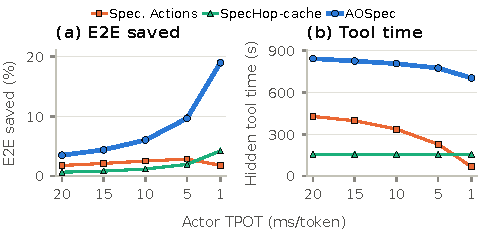
\includegraphics[width=\linewidth]{figs/swe_generalization}
\caption{SWE-bench transfer with the observation model trained on Terminal-Bench: (a) end-to-end latency savings and (b) total tool time hidden
across actor TPOTs.}
\label{fig:swe-generalization}
\end{figure}

\begin{figure*}[t]
\centering
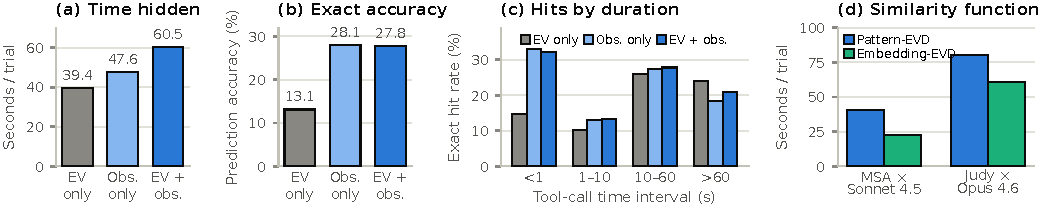
\includegraphics[width=\textwidth]{figs/evd_ablations}
\caption{Expected-value decoding over MSA~$\times$~Sonnet 4.5 and Judy~$\times$~Opus 4.6 (width 1, 10\,ms TPOT): (a) hidden tool time, (b) exact-match accuracy, and (c) exact-match hit rate are averaged across cells; (d) compares mined- and embedding-based value estimates for each cell.}
\label{fig:evd-ablations}
\end{figure*}

\begin{figure}[t]
\centering
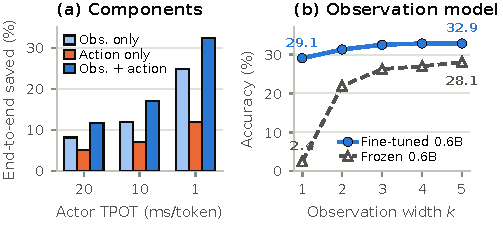
\includegraphics[width=\linewidth]{figs/component_ablation}
\caption{Component and observation-model ablations. (a) Mean latency savings
from observation speculation, action speculation, and their combination across nine Terminal-Bench cells. (b) Observation accuracy for fine-tuned and frozen 0.6B models on the same MSA$\times$Sonnet trials.}
\label{fig:component-ablations}
\end{figure}

\begin{figure}[t]
\centering
\begin{minipage}{0.49\textwidth}
\centering
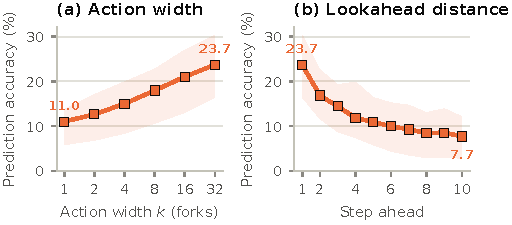
\includegraphics[width=\linewidth]{figs/mechanism_ablation}
\caption{Action-model ablations across nine Terminal-Bench cells:
trace-matched action accuracy versus (a) candidate width and (b) lookahead
distance. Curves show the nine-cell means; bands show the interquartile
ranges.}
\label{fig:action-model-ablations}
\end{minipage}
\end{figure}


\subsection{Experimental Setup}

\paragraph{Benchmarks and metrics.}
We evaluate \sysname{} through trace replay on Terminal-Bench
2.0~\citep{terminalbench2} and SWE-bench Verified~\citep{jimenez2024swebench},
spanning four agent harnesses---mini-swe-agent (MSA)~\citep{yang2024sweagent},
OpenHands~\citep{wang2025openhands}, Gemini CLI~\citep{geminicli2025}, and
Judy\footnote{Judy is an anonymous submission listed on the Terminal-Bench 2.0
leaderboard.}---and five actor models and nine harness--model configurations on
Terminal-Bench 2.0, plus MSA on SWE-bench Verified with traces from the
official ``Bash Only'' leaderboard.
We split Terminal-Bench tasks into disjoint training and test sets, ensuring
that every task category is represented in the test set. Predictors use only
training tasks.
Because the actors are accessed through APIs as black boxes
and all optimizations operate within the harness, live scheduling could cause methods to follow different trajectories.
We therefore follow the community convention to replay all methods on identical actor trajectories~\citep{xia2026idleness}, enabling reproducible comparisons across serving regimes.
We compute actor latency from recorded output token counts and sweep TPOT over
$\{20,15,10,5,1\}$\,ms/token, spanning conventional to low-latency serving
regimes~\citep{artificialanalysis_anthropic, artificialanalysis_openai, groq2024specdec, cerebras2025k2think}.
We primarily report total latency reduction relative to serial execution, alongside tool time hidden and exact prediction rate.

\paragraph{Baselines.}
We compare against Speculative Actions (\emph{Spec-Actions}), which uses
Qwen3.6-35B-A3B-FP8~\citep{qwen36_35b_a3b} to predict and launch the next
action~\citep{ye2025speculative}, and two Speculative Observation baselines, the SpecHop variants~\citep{saberi2026spechop}:
\emph{SpecHop-cache} reuses prior observations, while \emph{SpecHop-LLM} uses
Qwen3.6-35B-A3B-FP8 to draft observations. 
\emph{Oracle-action} receives the correct next action from the trace and defines the one-step action speculation ceiling. 
Serial execution is the vanilla baseline.

\paragraph{Hardware.}
Drafter generation runs on 2 NVIDIA H200 GPUs.
Tool calls are run on a Microsoft Azure Standard\_D4s\_v5 VM.
The VM has four vCPUs and 16\,GiB of memory with an Intel Xeon Platinum 8370C (Ice Lake) processor at 2.80\,GHz. Storage consists of a 64\,GB Premium SSD OS disk and a 256\,GB P15 Premium SSD data disk.

\paragraph{Implementation.}
The observation drafter is Qwen3-0.6B, fine-tuned for each harness.
The action drafter is Qwen3.6-35B-A3B-FP8 without additional training.
vLLM~\citep{kwon2023efficient} is used as the serving backend for drafting.
Unless stated otherwise, \sysname{} uses five observation branches and eight action forks.

\subsection{End-to-End Performance and Tail Latency}

\paragraph{Comparison with baselines.}
As shown in Figure~\ref{fig:main-results}, \sysname{} outperforms every
practical baseline across all 45 configuration and TPOT combinations. Its
mean saving across equally weighted configurations rises from 11.8\% at
20\,ms TPOT to 32.5\% at 1\,ms, compared with 4.3\% and 12.2\% for the
strongest baseline. Spec-Actions provides negligible savings in most
settings because long tool executions overlap only with much shorter actor
decodes. SpecHop-cache performs well when observations recur, particularly
with Gemini 2.5 Pro under MSA and OpenHands and in the Judy configurations,
but offers little benefit for Gemini CLI and most GPT-5 mini settings, where
costly outputs are less reusable. In contrast, \sysname{} remains effective
across all configurations. It also exceeds the one step action oracle in 41
of 45 settings because observation speculation and cross step action
lookahead extend beyond the one step action only ceiling. Its advantage grows
as faster decoding exposes more tool time while reducing same step overlap.

\paragraph{Tail latency.}
Table~\ref{tab:latency-distribution} reports trial-level latency at the representative 10\,ms TPOT. 
\sysname{} achieves the lowest latency at every reported quantile. It
reduces median and p90 latency by 10.7\% and 10.5\%, while the reductions grow
to 30.3\% at p95 and 42.8\% at p99. The larger tail gains agree with the
latency concentration identified in Section~\ref{sec:challenge1}.

\begin{table}[t]
\centering
\setlength{\tabcolsep}{3.0pt}
\caption{End-to-end latency distribution (seconds) per trial
at 10\,ms actor TPOT.}
\label{tab:latency-distribution}
\resizebox{\columnwidth}{!}{%
\begin{tabular}{@{}lrrrrrr@{}}
\toprule
Method & p10 & p30 & p50 & p90 & p95 & p99 \\
\midrule
Serial         & 56 & 129 & 229 & 1038 & 1842 & 7780 \\
Spec-Actions & 56 & 129 & 226 & 1036 & 1812 & 7765 \\
SpecHop-cache  & 55 & 129 & 223 & 1003 & 1624 & 5052 \\
SpecHop-LLM    & 55 & 128 & 223 & 1008 & 1779 & 7449 \\
Oracle-action  & 53 & 124 & 220 & 971  & 1669 & 7750 \\
\sysname{}     & \textbf{49} & \textbf{114} & \textbf{204} &
                 \textbf{929} & \textbf{1285} & \textbf{4449} \\
\midrule
\sysname{} reduction (\%) & 12.1 & 11.1 & 10.7 & 10.5 & 30.3 & 42.8 \\
\bottomrule
\end{tabular}
}
\end{table}

\subsection{Generalization to an Unseen Benchmark}

Figure~\ref{fig:swe-generalization} evaluates SWE-bench using the observation
model trained only on Terminal-Bench traces. At 1\,ms TPOT, \sysname{} achieves
18.9\% latency savings, compared with 4.2\% for the strongest baseline,
demonstrating transfer to an unseen benchmark without retraining.

\subsection{Expected-Value Decoding Targets Costly Calls}

\paragraph{Effect of latency weighting.}
Figure~\ref{fig:evd-ablations}(a--b) compares three decoding rules over
candidates from the same observation model: estimated tool time, model
likelihood, and their EVD product. Tool time alone favors costly but
implausible outcomes, whereas likelihood favors probable outcomes regardless
of their latency. By balancing both, EVD hides 60.5 seconds per trial, versus
47.6 seconds for likelihood and 39.4 seconds for tool time.
It redirects correct predictions toward
costly calls, raising the hit rate above 60 seconds from 18.4\% to
21.0\% while slightly reducing it for subsecond calls
(Figure~\ref{fig:evd-ablations}(c)). Thus, EVD hides more time without
requiring more correct predictions.

\paragraph{Similarity function.}
Figure~\ref{fig:evd-ablations}(d) compares two implementations of $K$:
\emph{Pattern-EVD} groups observations matched by the same mined regular
expression pattern, whereas \emph{Embedding-EVD} groups observations that are
nearby in a learned representation space. Pattern-EVD hides 40.9 versus 22.3
seconds per trial on MSA~$\times$~Sonnet 4.5 and 80.1 versus 61.2 seconds on
Judy~$\times$~Opus 4.6. We therefore use Pattern-EVD in the main evaluation.

\subsection{Ablation Studies}

\paragraph{Two-level speculation.}
Figure~\ref{fig:component-ablations}(a) shows that, at 10\,ms TPOT,
observation and action speculation alone save 12.0\% and 7.1\% on average,
respectively, while their combination saves 17.0\%. At 1\,ms TPOT, the joint
savings reach 32.5\%. The two levels are complementary: observation
speculation advances generation past predictable observations, while action
speculation executes tools early to resolve environment-dependent outputs.

\paragraph{Observation-model training.}
On the same MSA$\times$Sonnet trials, fine-tuning the 0.6B observation model
raises top-1 accuracy from 2.4\% to 29.1\%
(Figure~\ref{fig:component-ablations}(b)). 
As candidate width increases to
five, however, the frozen model reaches 28.1\% versus 32.9\% for the
fine-tuned model, narrowing the gap from 26.7 to 4.8 percentage points. 
This convergence suggests that, with sufficient compute for multiple attempts, \sysname{} can operate training-free using an off-the-shelf observation model.

\paragraph{Action-speculator accuracy.}
Increasing candidate width from 1 to 32 raises mean trace-matched accuracy
from 11.0\% to 23.7\%, trading additional forks for greater coverage
(Figure~\ref{fig:action-model-ablations}(a)). At width 32, target-action
accuracy declines from 23.7\% at distance one to 7.7\% at distance ten
(Figure~\ref{fig:action-model-ablations}(b)). By verifying the target action
and its launch state directly, JASV keeps these long-range predictions usable
without requiring the intervening action chain to match, whose accuracy is
effectively zero at this distance.

\subsection{Observation-Model Context}

\begin{table}[t]
\centering
\small
\setlength{\tabcolsep}{5pt}
\caption{Observation model input ablation on MSA~$\times$~Sonnet 4.5. Each variant removes the indicated component during both training and inference; history contains all prior reasoning, tool calls, and observations.}
\label{tab:observation-input-ablation}
\begin{tabular}{@{}lcc@{}}
\toprule
Removed input & \shortstack{Tool time\\hidden (\%)} &
\shortstack{Exact hit\\rate (\%)} \\
\midrule
None (full context)        & 27.1          & 33.3          \\
Task query                 & \textbf{28.7} & \textbf{33.6} \\
Reasoning text             & 27.3          & \textbf{33.6} \\
Prior observations         & 26.5          & 30.1          \\
All prior steps (history)  & 27.2          & 29.9          \\
\bottomrule
\end{tabular}
\end{table}

\paragraph{Effect of input components.}
As shown in Table~\ref{tab:observation-input-ablation}, removing the task query or reasoning text does not decrease both hit rate and tool time hidden.
Removing prior observations or the entire interaction history lowers exact hit rate from 33.3\% to 30.1\% and 29.9\%, respectively, while hidden time remains stable.
We therefore condition the observation model on the current action and
prior interaction history.
